\chapter{显示测试}
\section{字体测试}
中文宋体正常 \textbf{中文宋体加粗} \textit{中文宋体斜体}

English \textbf{English} \textit{English}
\section{数学公式测试}
带编号公式
\begin{equation}
    \int_0^1 x^2 \mathrm{d}x = \frac{1}{3}.
\end{equation}

不带编号公式
\begin{equation*}
    \int_0^1 x^2 \mathrm{d}x = \frac{1}{3}.
\end{equation*}

\section{图片测试}
单图测试
\begin{figure}[h]
    \centering
    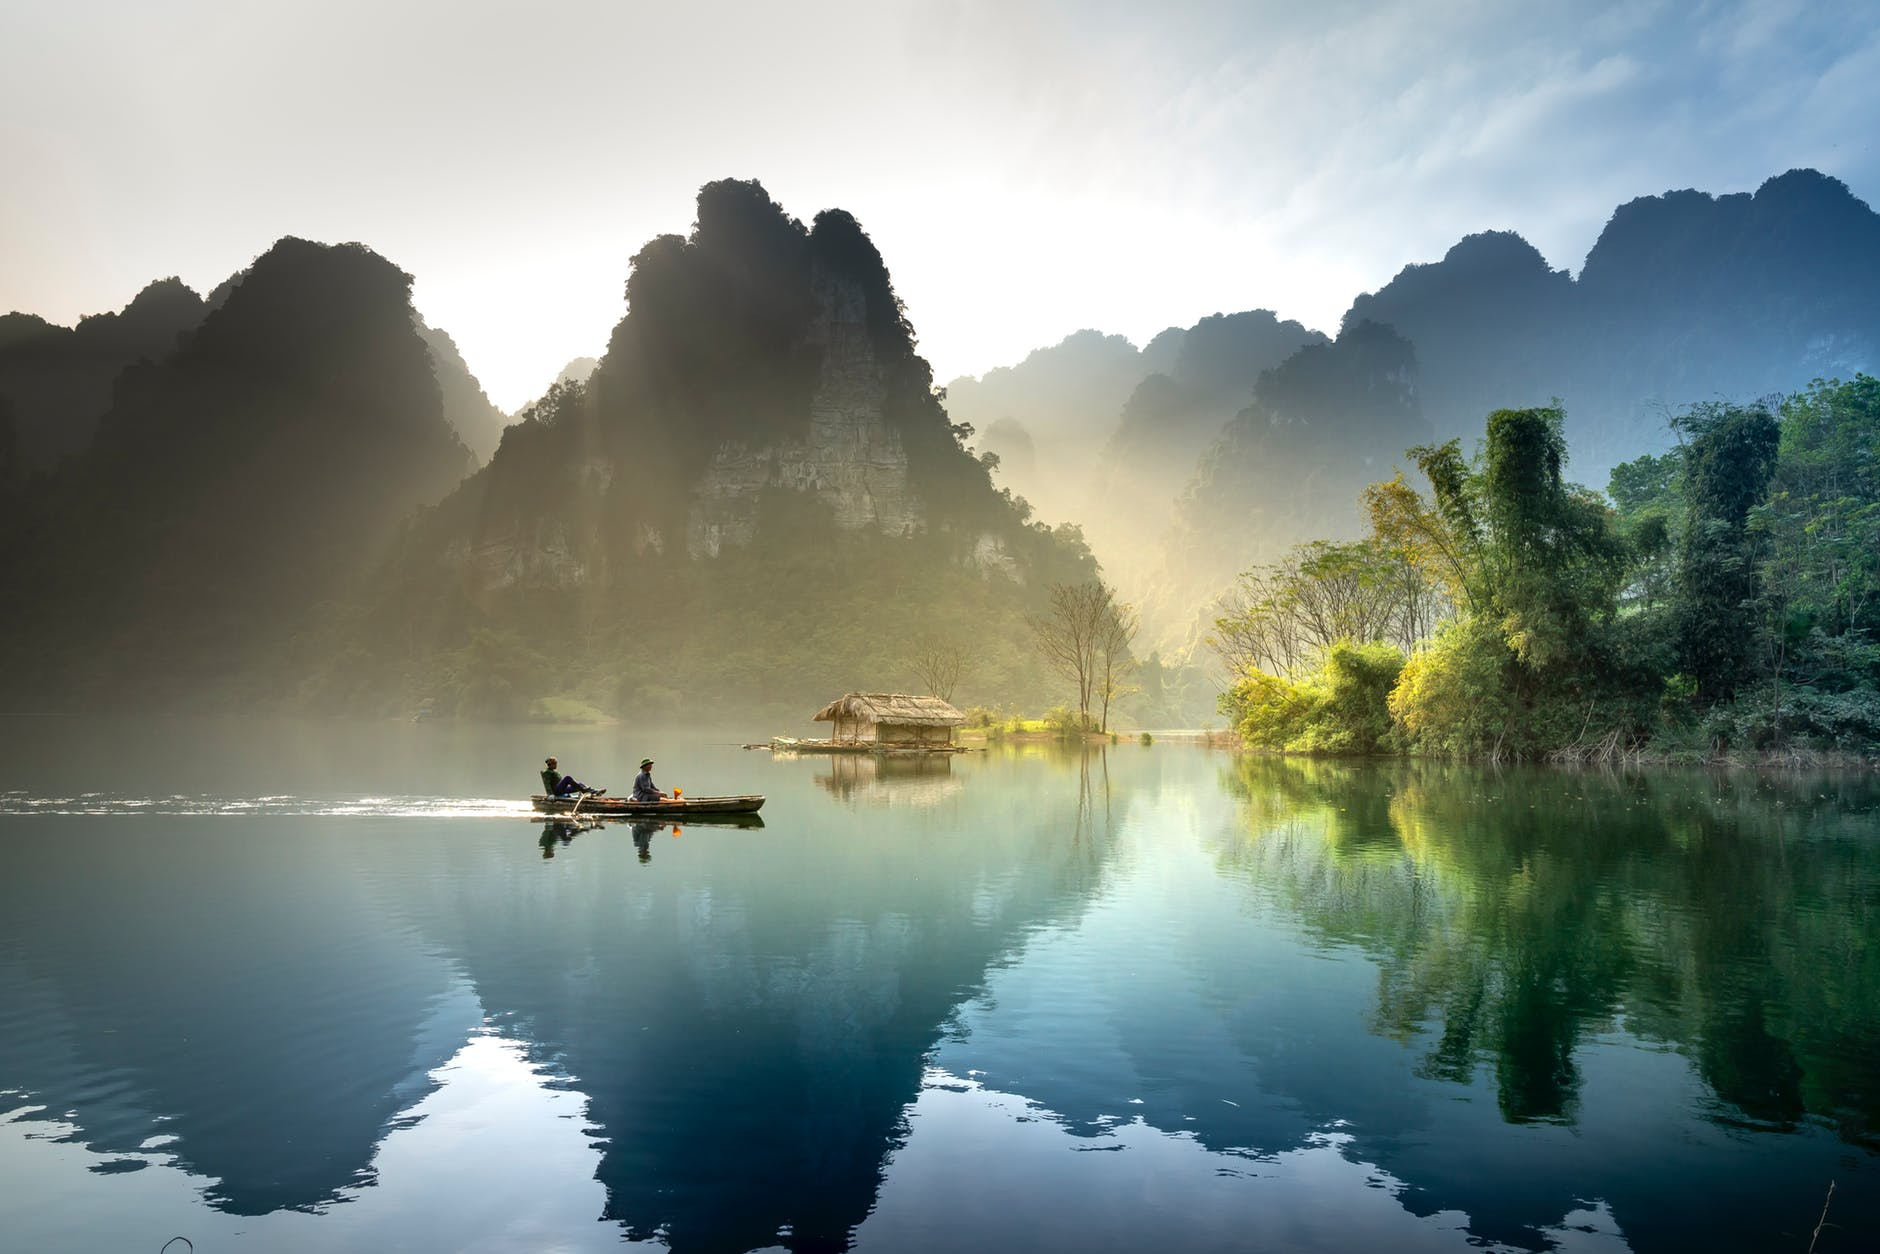
\includegraphics[width=0.8\textwidth]{lake.jpeg}
    \caption{单图片}
    \label{fig:singlePic}
\end{figure}

多图测试1
\begin{figure}[h]
    \centering
    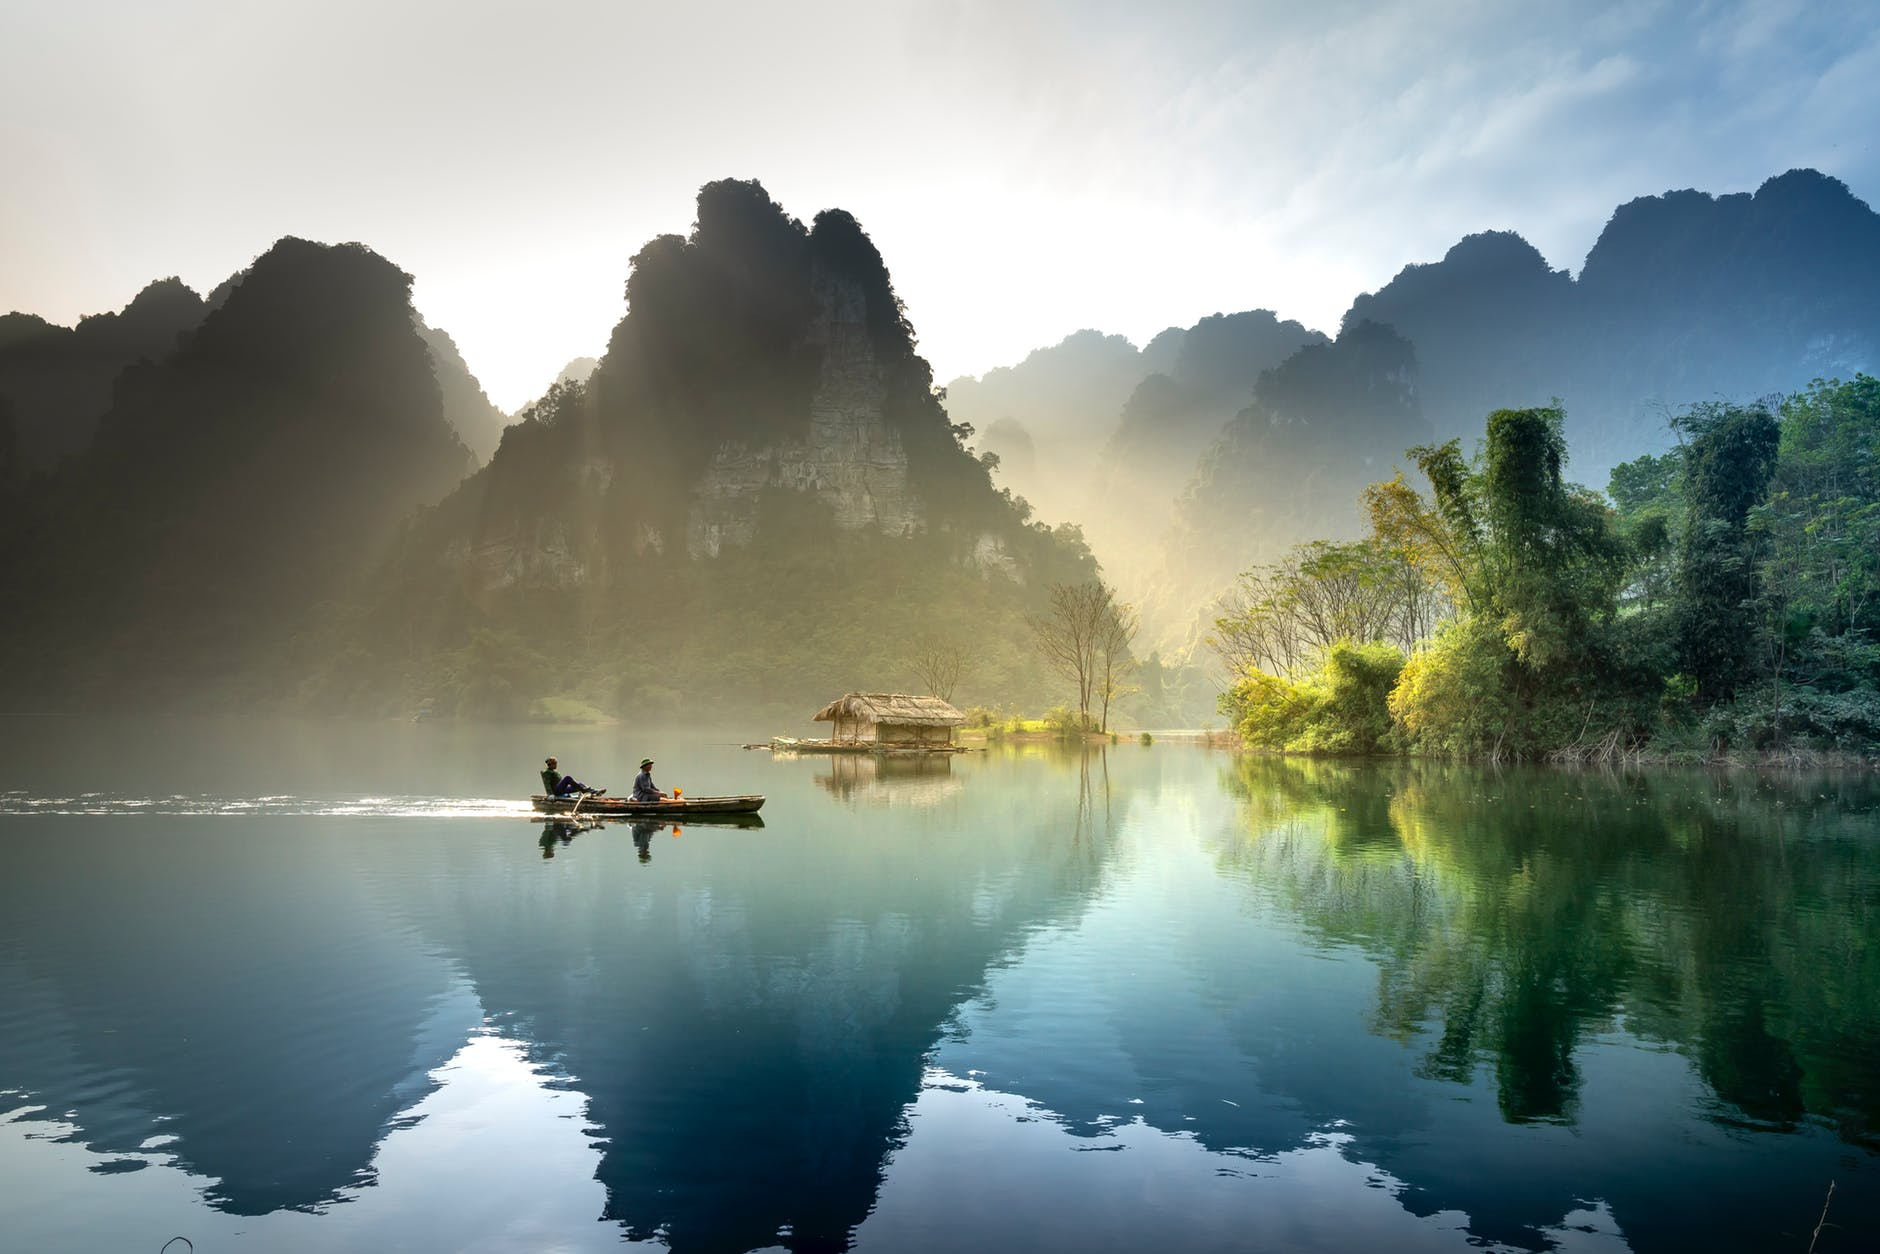
\includegraphics[width=0.3\textwidth]{lake.jpeg}\hfill
    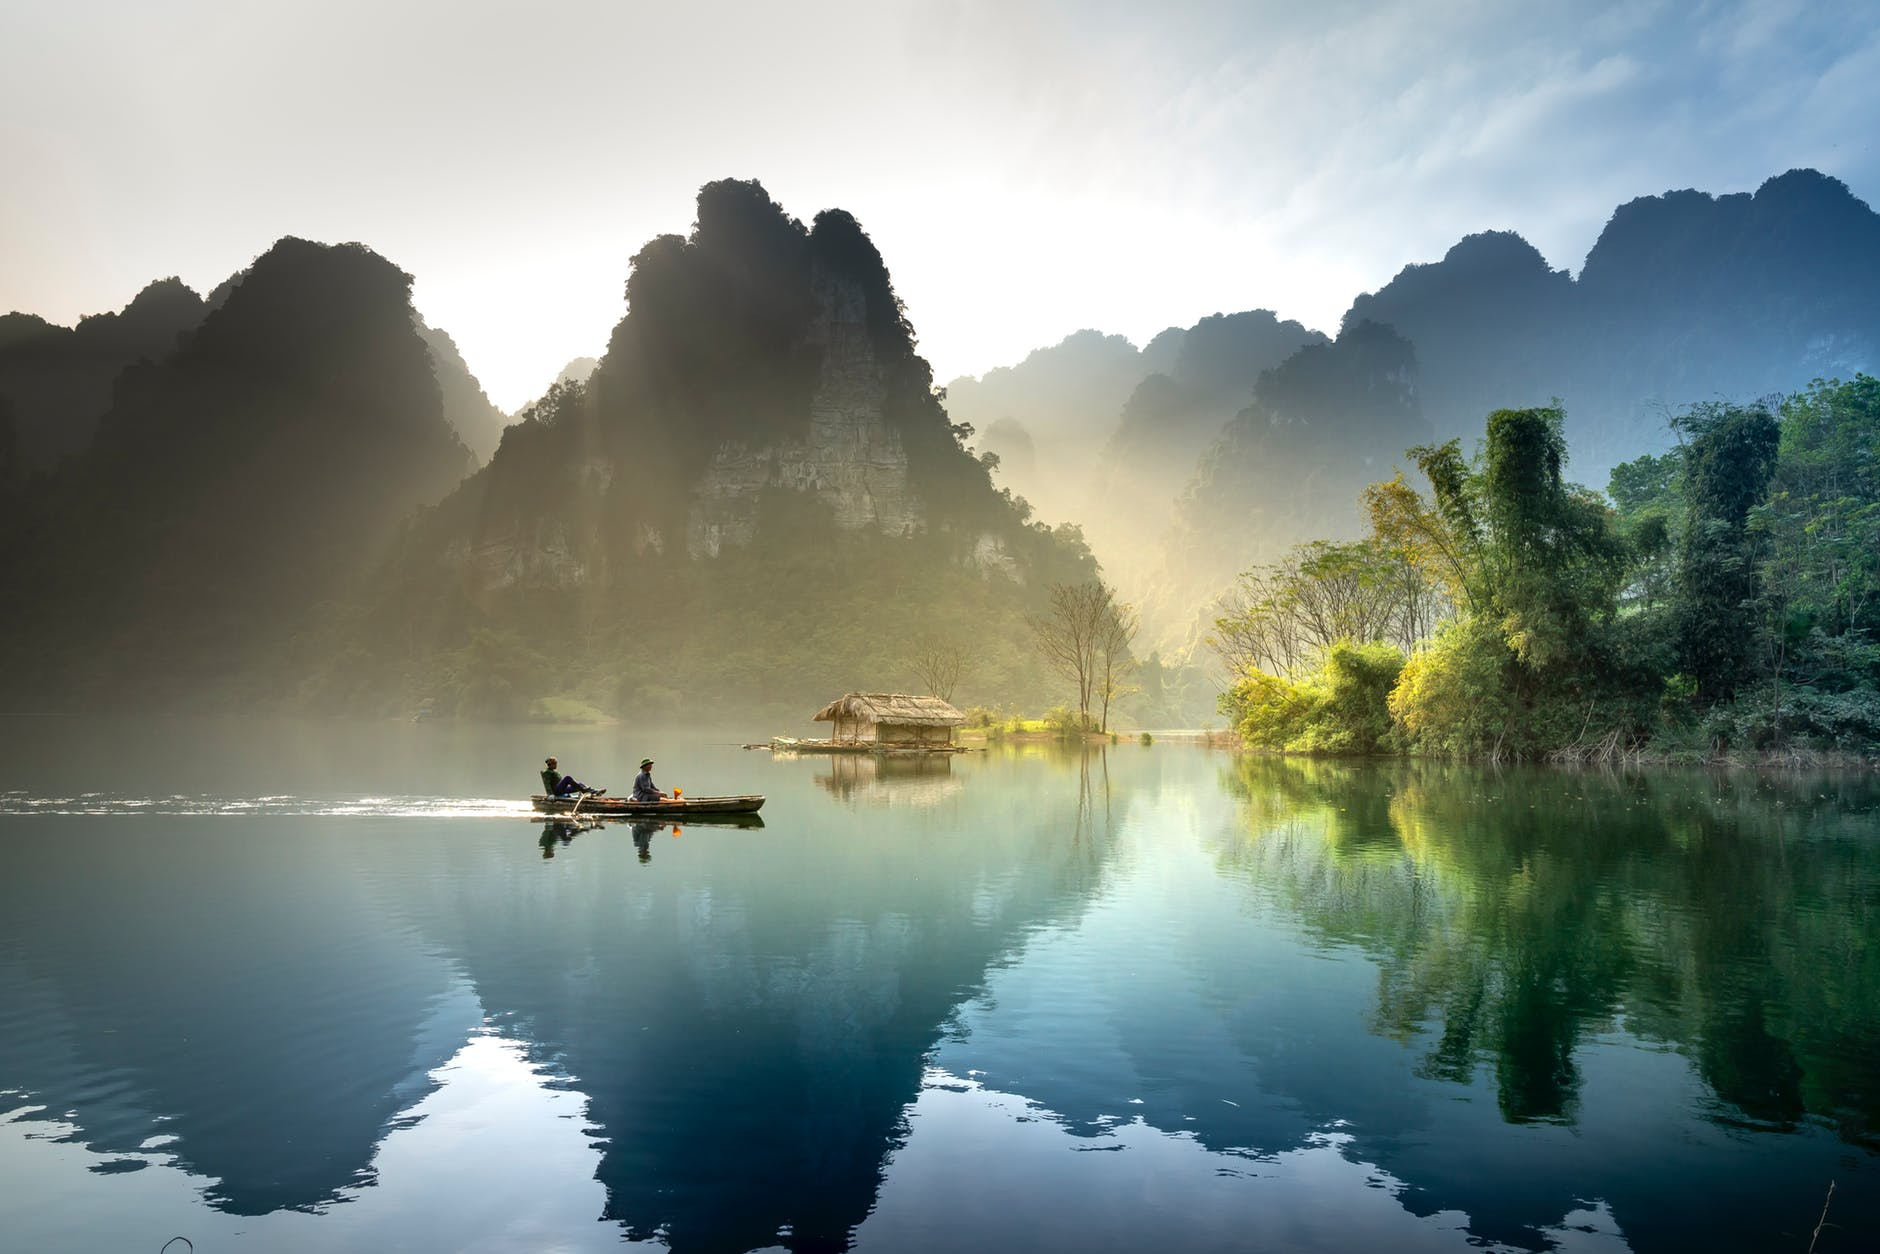
\includegraphics[width=0.3\textwidth]{lake.jpeg}\hfill
    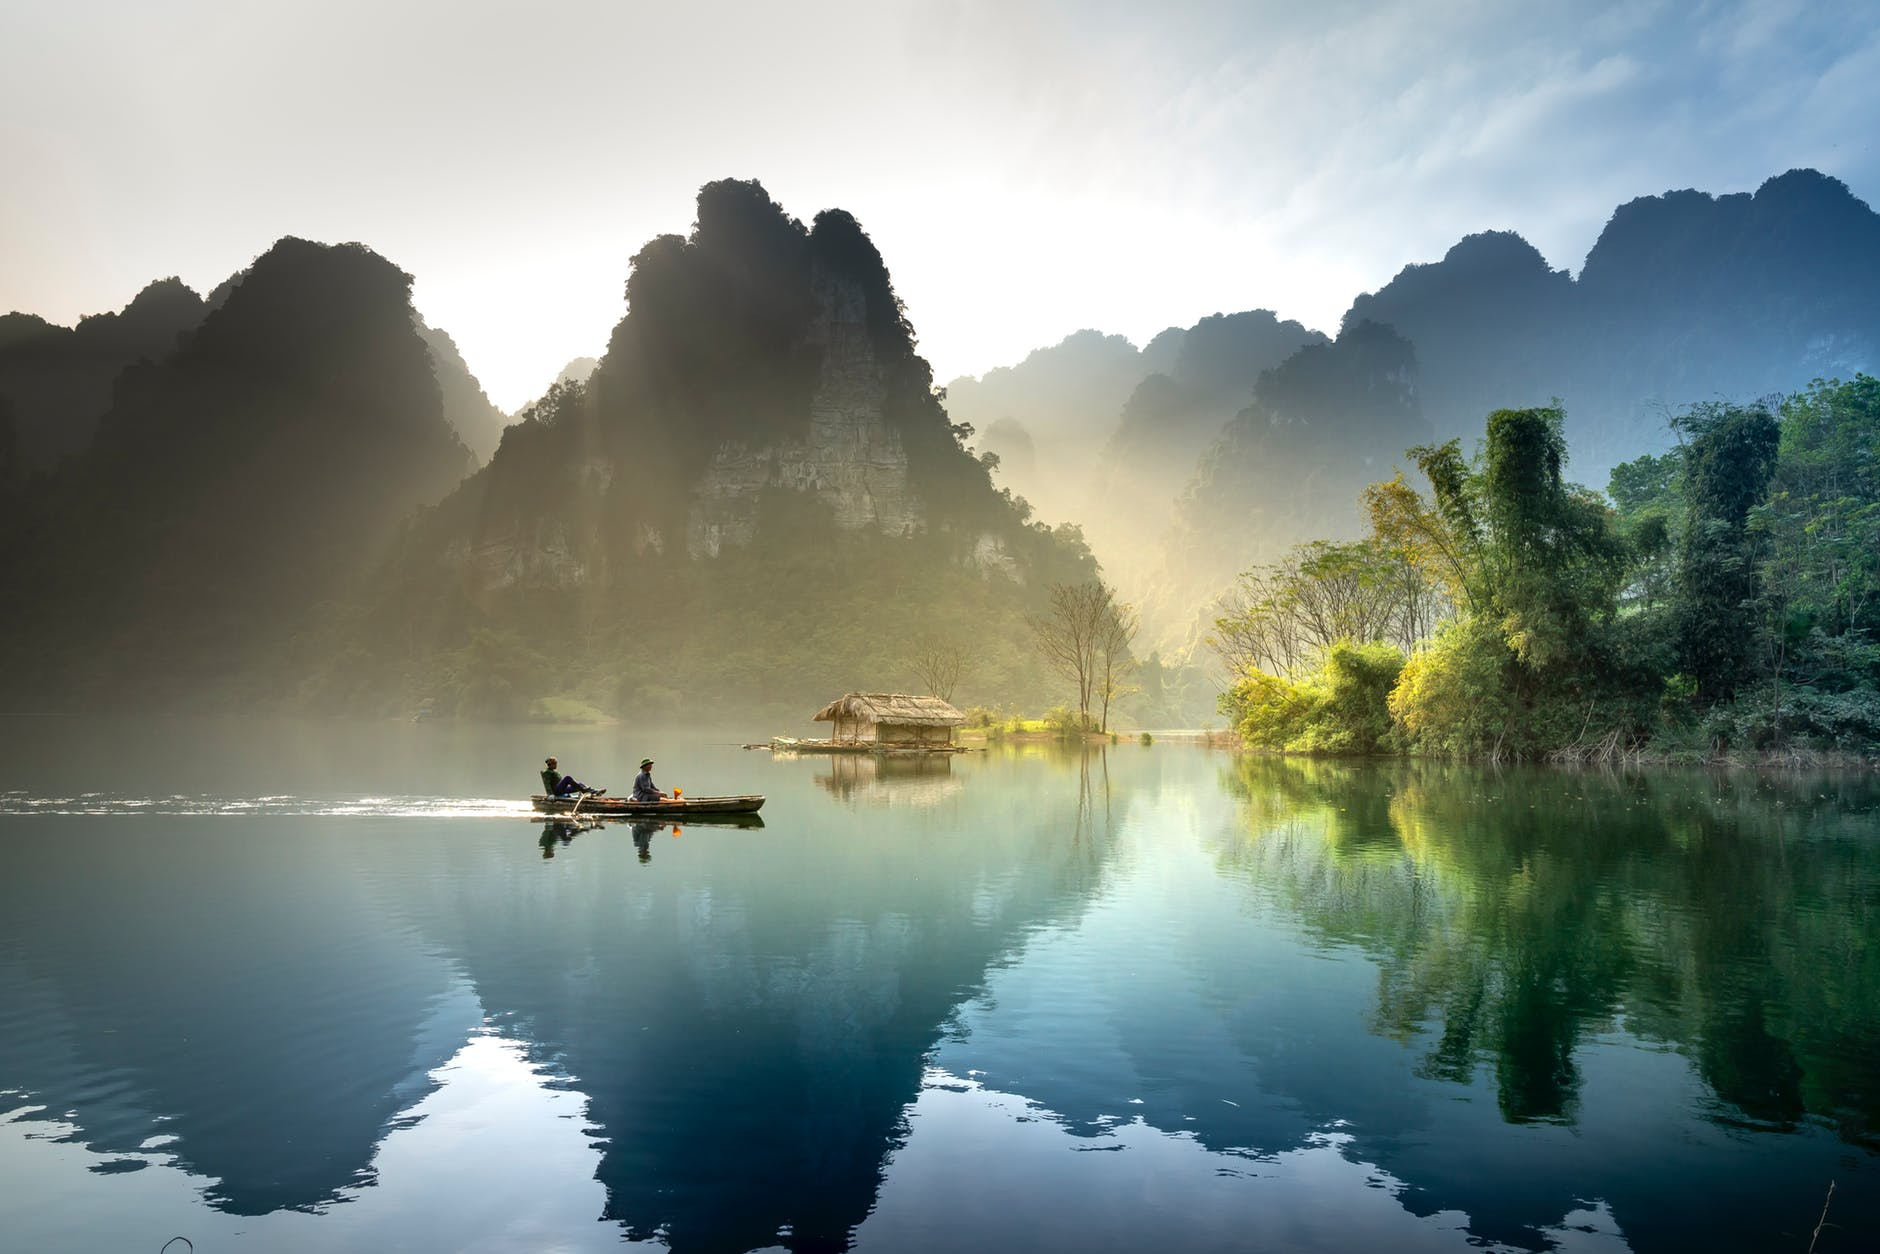
\includegraphics[width=0.3\textwidth]{lake.jpeg}
    \caption{多图片1:珠江三角洲投资管理体制市场化改革(1985---2005)}
    {\zihao{5} \songti 资料来源:xxx}
    \label{fig:MultiPic1}
\end{figure}

多图测试2
\begin{figure}[h]
    \centering
    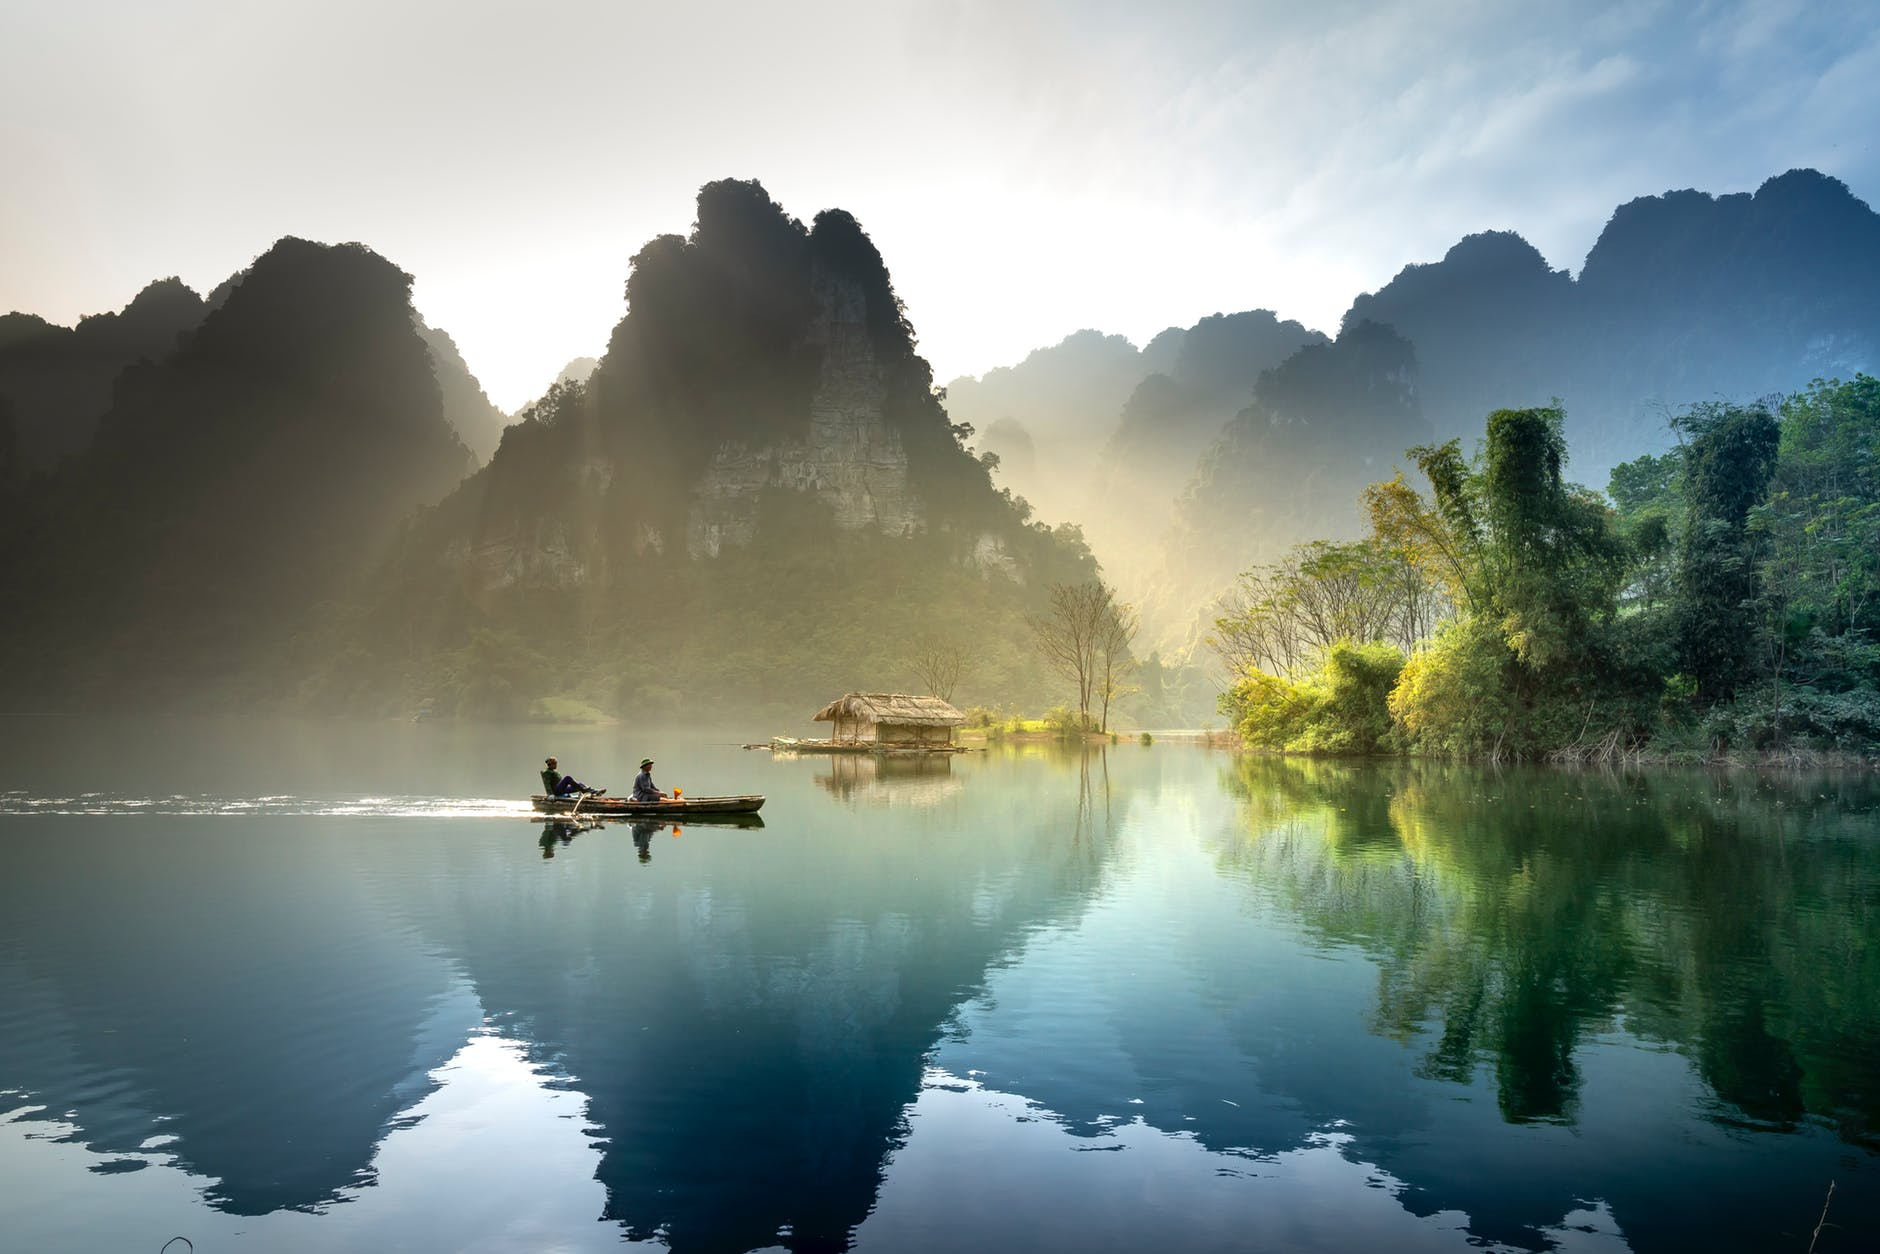
\includegraphics[width=0.5\textwidth]{lake.jpeg}\\
    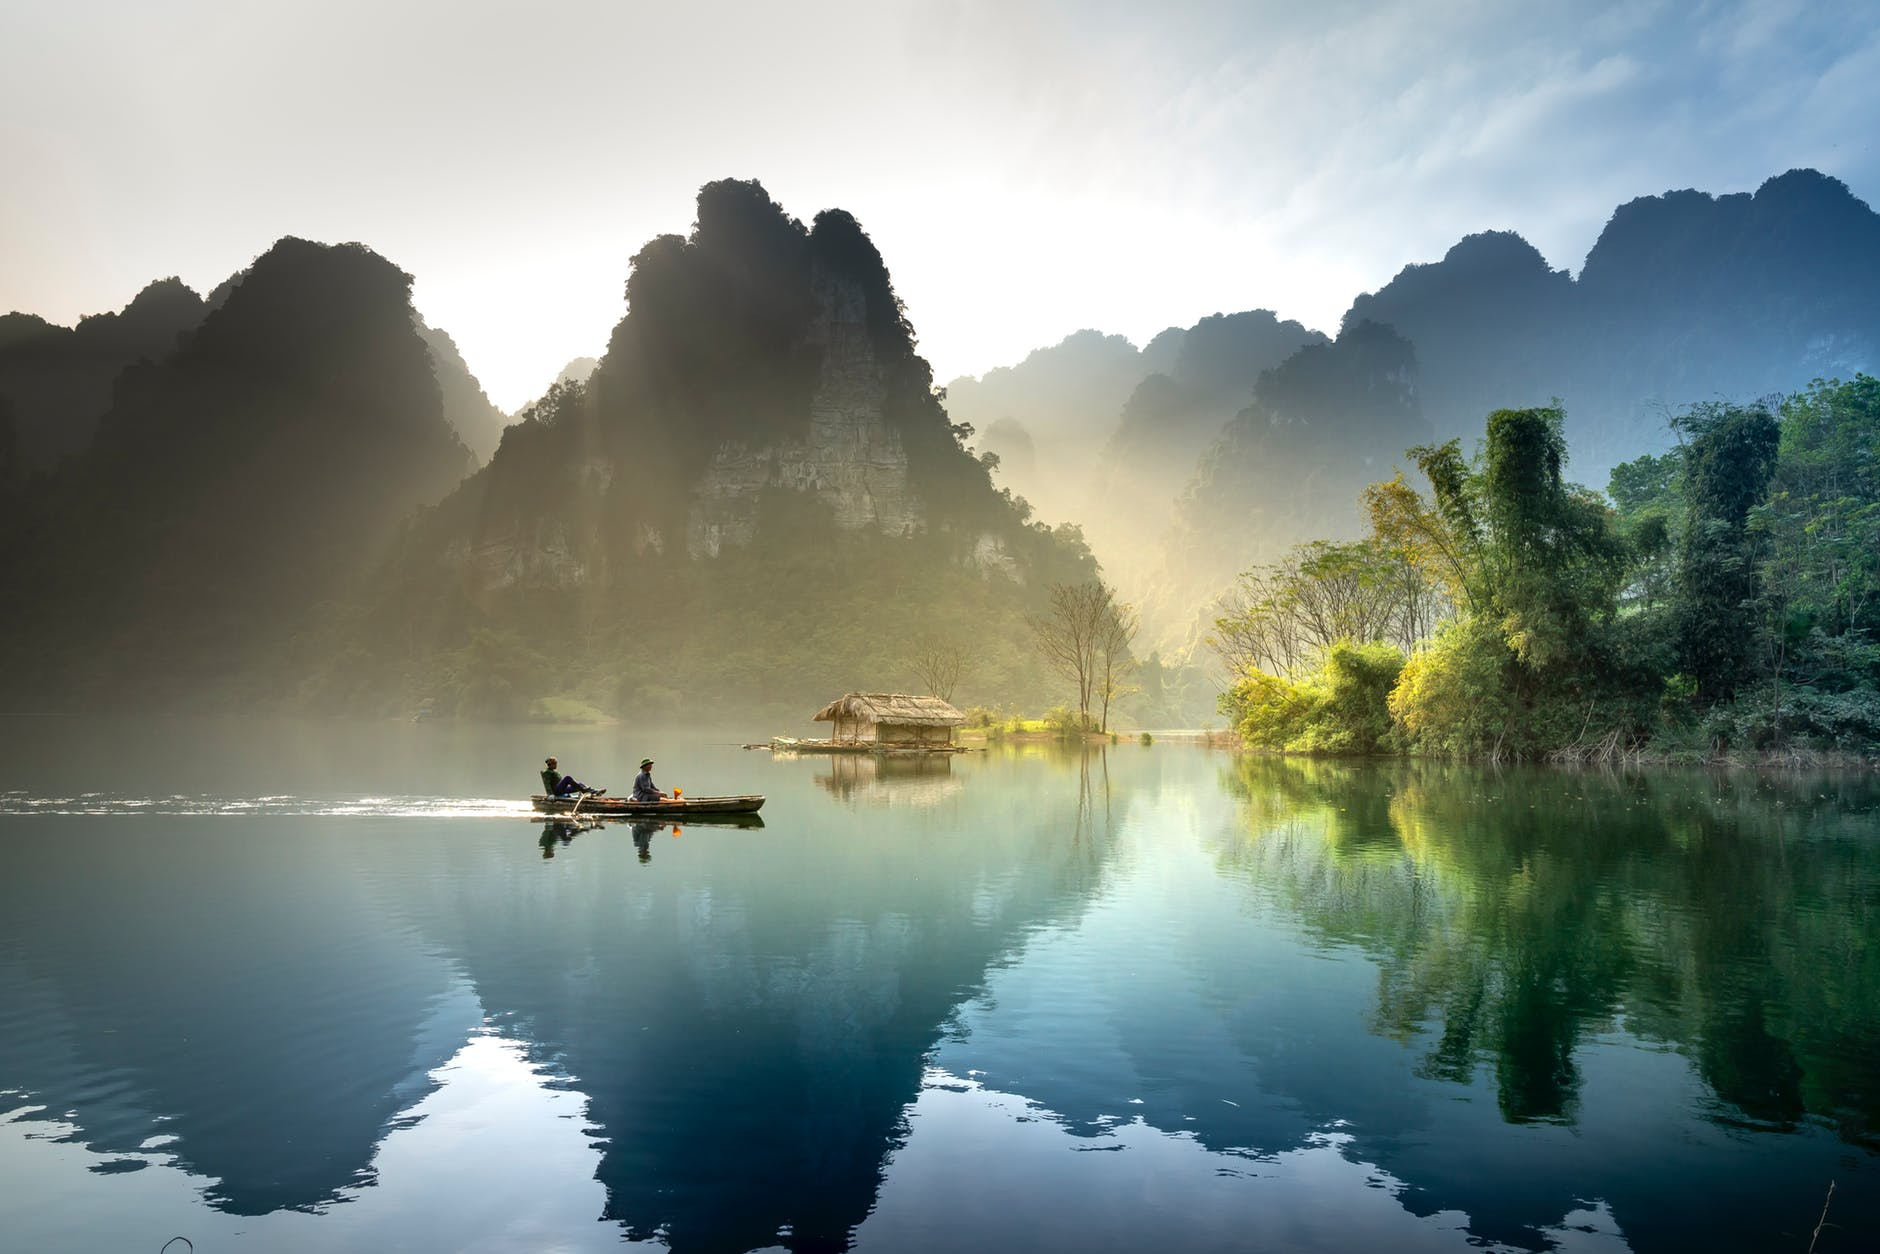
\includegraphics[width=0.5\textwidth]{lake.jpeg}\\
    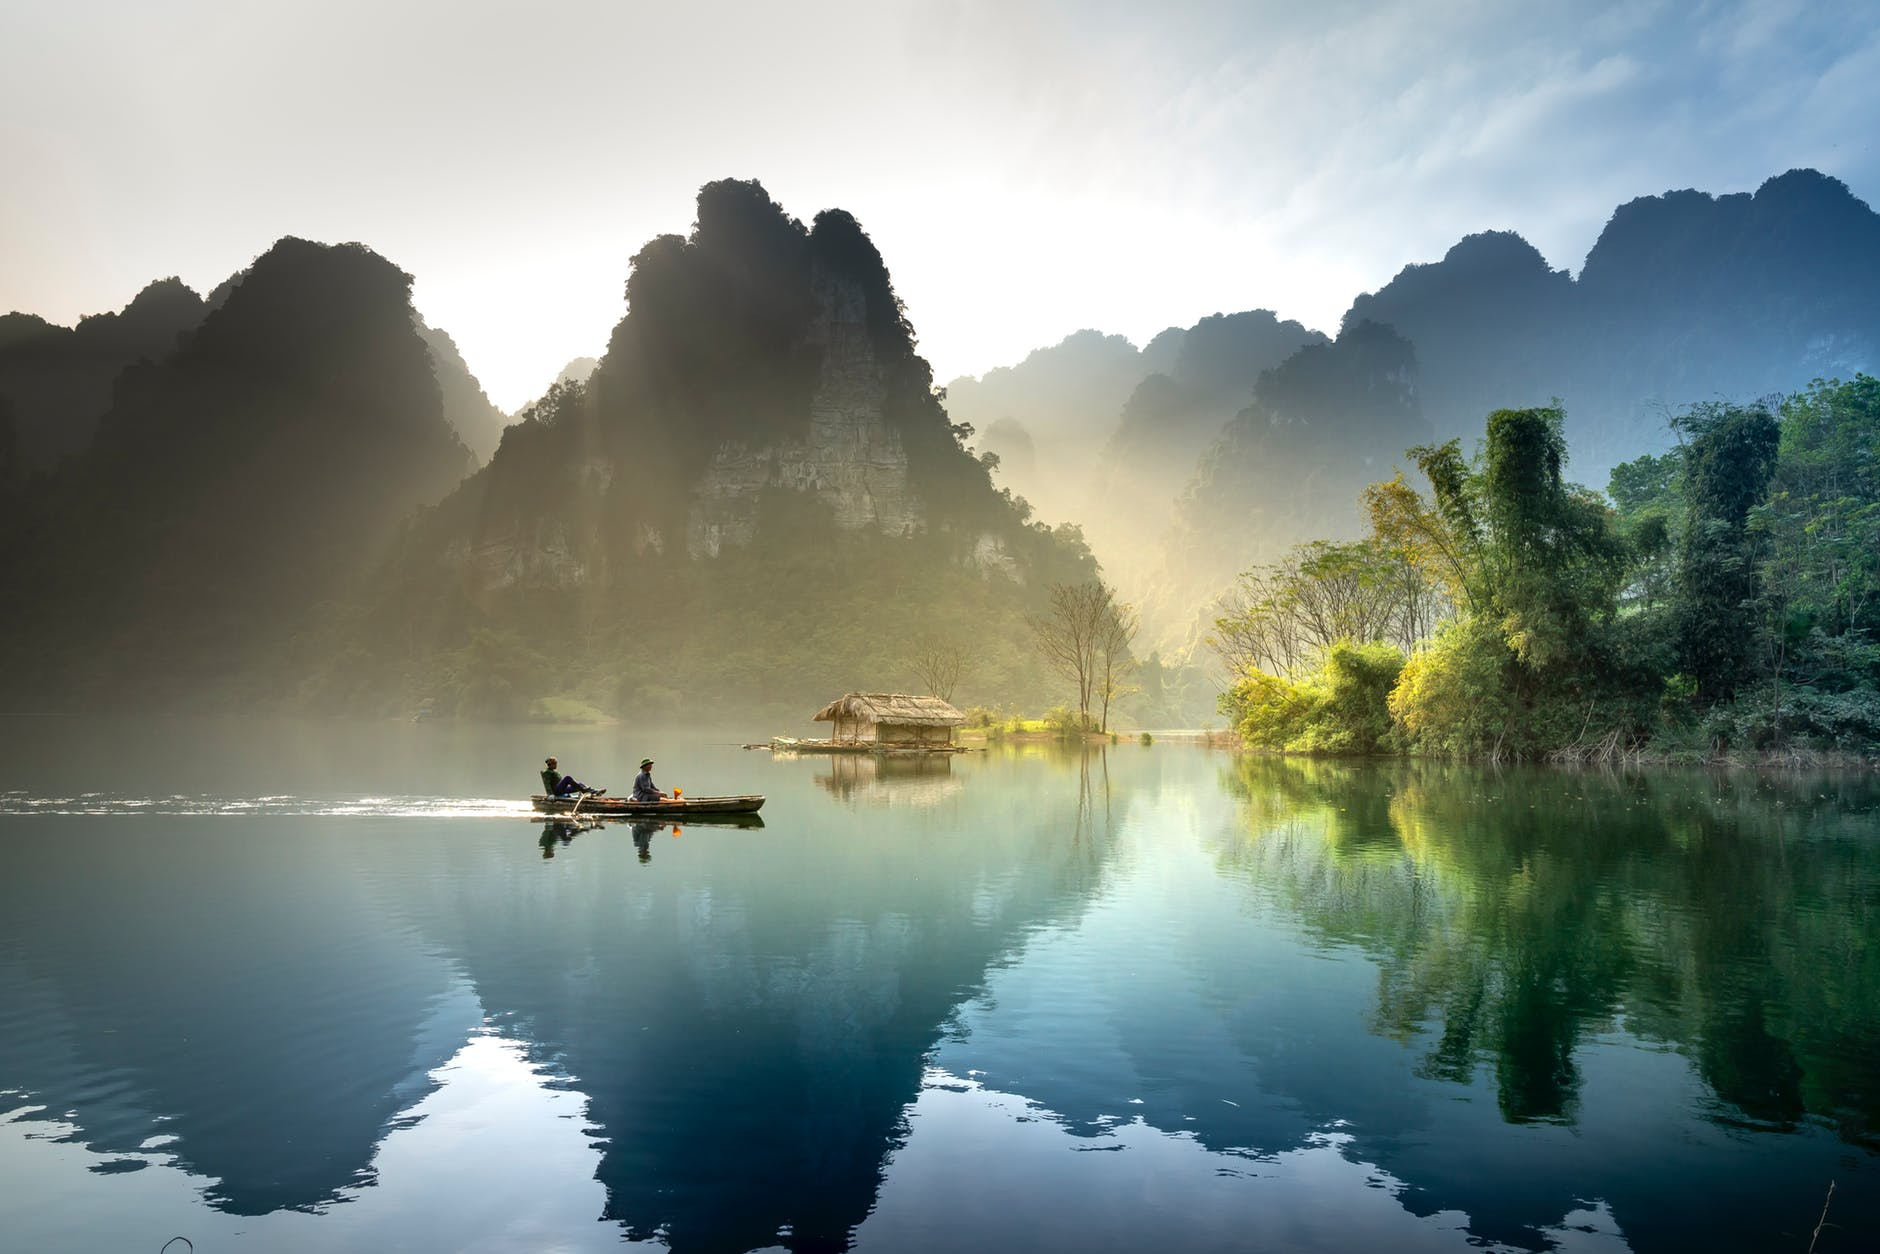
\includegraphics[width=0.5\textwidth]{lake.jpeg}
    \caption{多图片2}
    \label{fig:MultiPic2}
\end{figure}
